\documentclass[journal,twocolumn]{IEEEtran}

\usepackage[utf8]{inputenc}
\usepackage{graphicx}
\usepackage{amssymb}
\usepackage{amsmath}
\providecommand{\pr}[1]{\ensuremath{\Pr\left(#1\right)}}
\providecommand{\cbrak}[1]{\ensuremath{\left\{#1\right\}}}

\title{Assignment 4}
\author{Gollapudi Sasank CS21BTECH11019}

\begin{document}
\maketitle
\section*{Question : }
In a factory which manufactures bolts, machines A, B and C manufacture
respectively 25\% , 35\% and 40\% of the bolts. Of their outputs, 5, 4 and 2 percent are respectively defective bolts. A bolt is drawn at random from the product and is found to be defective. What is the probability that it is manufactured by the machine B?
\section*{Solution : }
Let  events $B_1,B_2,B_3$ be the following : \\
$B_1$ : the bolt is manufactured by machine A \\
$B_2$ : the bolt is manufactured by machine B \\
$B_3$ : the bolt is manufactured by machine C \\
A bolt must be manufactured from exactly one of the machines A,B,C.\\
Therefore $B_1,B_2,B_3$ are mutually exclusive and exhaustive events and hence, they represent a partition of the sample space.
Let the event $E$ be `the bolt is defective'.\\
The event $E$ occurs with $B_1$ or with $B_2$ or with $B_3$.\\
Given that 
\begin{align}
\pr{B_1} &= 25\% = 0.25 \\
\pr{B_2} &= 35\% = 0.35 \\
\pr{B_3} &= 40\% = 0.4 
\end{align} 
And also $\pr{E|B_1} = $ Probability that the bolt drawn is defective given that the bolt is manufactured from machine A $ = 5\% = 0.05 $ \\
Similarly
\begin{align}
\pr{E|B_1} &= 5\% = 0.05 \\
\pr{E|B_2} &= 4\% = 0.04 \\
\pr{E|B_3} &= 2\% = 0.02
\end{align}
We need to find the Probability that bolt is manufactured by $B_2$, Given that the bolt is defective i.e  the value of $\pr{B_2|E}$ \\
From Bayes Theorem , \\
\begin{align}
\pr{B_2|E} &= \frac{\pr{B_2}\pr{E|B_2}}{\pr{B_1}\pr{E|B_1}+\pr{B_2}\pr{E|B_2}+\pr{B_3}\pr{E|B_3}} \\
\Rightarrow \pr{B_2|E} &= \frac{0.35 \times 0.04}{0.25 \times 0.05 + 0.35 \times 0.04 + 0.4 \times 0.02 } \\
\Rightarrow \pr{B_2|E} &= \frac{0.014}{0.0125+0.014+0.008} \\
\Rightarrow \pr{B_2|E} &= \frac{0.014}{0.0345} \\ 
\Rightarrow \pr{B_2|E} &= \frac{28}{69} \\ 
\therefore \pr{B_2|E} &= \frac{28}{69} = 0.4058 
\end{align}
\begin{figure}[h]
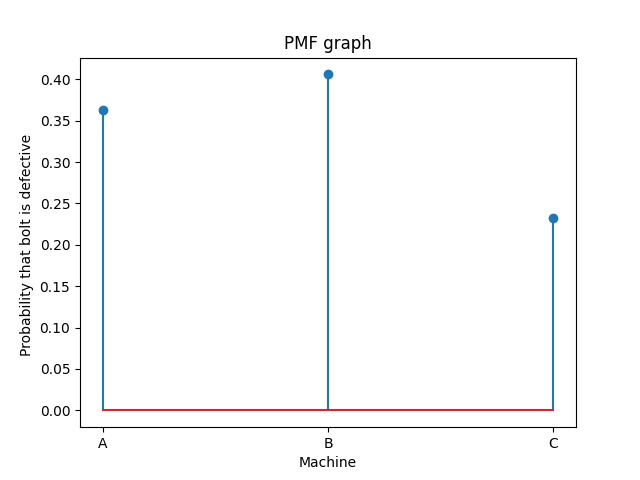
\includegraphics[width=\columnwidth]{Fig-1.png}
\caption{PMF graph}
\label{Fig 1}
\end{figure}
\end{document}
